
\chapter{Using SystemVerilog for Digital Design Education}
\label{chapter:digital_design}

Navigating the realm of Verilog/SystemVerilog education presents a distinctive challenge: effectively bridging the gap between abstract Verilog syntax and tangible hardware implementations. Striking this balance is of paramount importance, as it can equip aspiring electrical engineers with a deep comprehension of digital circuits, while giving them the hard-skills in computer-aided circuit creation. While it may feel there is a tradeoff between teaching Verilog design strategies and teaching circuit design strategies, I argue that teaching inference and synthesis of Verilog will actually augment student understanding of more advanced digital circuit concepts. I would compare this to a programming course using C++ to teach algorithms. For many computer science students, algorithms are synonymous with code, not with logic proofs. For computer engineering students, \ul{as long as Verilog is taught with a synthesis-oriented approach, the connection between theoretical circuit concepts and tangible hardware construction becomes seamless, facilitating a more rapid and all-encompassing digital design education.}

\section{Netlist graph viewers teach Verilog inference intuition.}


\begin{figure}[t]
    \centering
    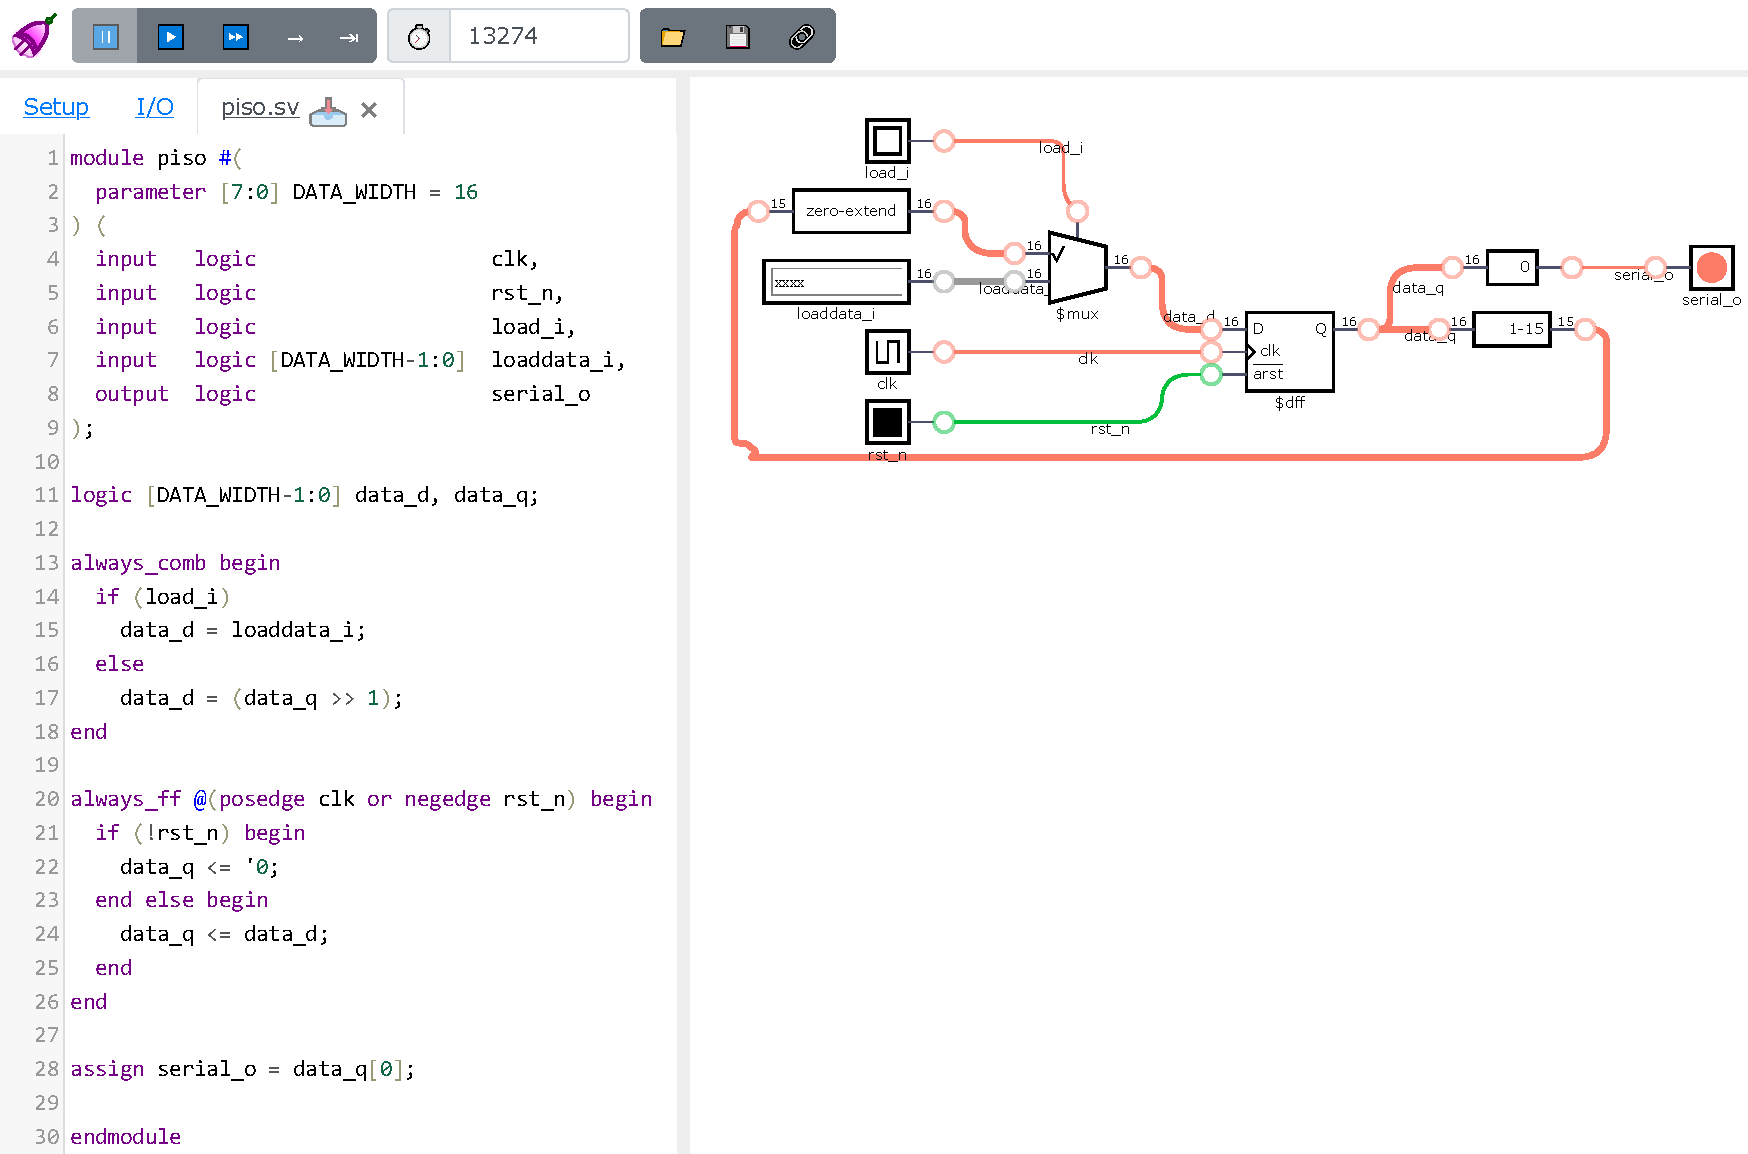
\includegraphics[width=\linewidth]{figures/digitaljs_online.pdf}
    \caption{Schematic for a Parallel-in Serial-out shift register generated by the netlist graph viewer DigitalJS Online \cite{DigitalJSOnline}}
    \label{fig:digitaljs_online}
\end{figure}


By using netlist graph viewers to provide a visual representation of the synthesis process, students can gain a deeper insight into how their high-level descriptions are transformed into hardware components. DigitalJS Online \cite{DigitalJSOnline} stands as a notable example of such netlist graph viewers. Through its zero-setup, interactive web interface, students can witness rapid translation of their Verilog code into synthesized hardware, which encourages experimentation and rapid prototyping. Additionally, its text editor runs automatic linting with Verilator, which gives incredibly helpful feedback if a syntax-related bad-practice is detected. During a volunteer lecture for UCSB's IEEE student chapter, I taught Verilog concepts from DigitalJS Online's text editor, which seamlessly visualized the logic I was describing in my examples. Also, as a TA for ECE 152A and 154B, I curated several assignments that challenged students to use DigitalJS Online to transform \mintinline{systemverilog}{for} loops and \mintinline{systemverilog}{if} statements into comprehensive, hand-drawn circuit diagrams. \autoref{fig:digitaljs_online} Similarly, UC Santa Cruz Professor Dustin Richmond uses netlist graph viewers to teach best-practices concerning \mintinline{systemverilog}{case} and \mintinline{systemverilog}{if} statements. \cite{RichmondLatchUp} Through a process of hands-on exploration with netlist graph viewers, students can learn the mechanics of translating SystemVerilog constructs into tangible hardware and gain the ability to convert Verilog to schematics by hand. By assigning homework and in-lecture exercises that prompt students to deduce logical constructs from visual synthesis outputs, their aptitude to understand both Verilog and synthesis is significantly enhanced.

\FloatBarrier

\section{Enabling optimizations in netlist graph viewers creates complexity.}
\label{section:optimizations_in_netlist_graph_viewers}


\begin{figure}[t]
    \centering

    \subfloat[
        If any bits of \mintinline{systemverilog}{a} are set, then \mintinline{systemverilog}{out} is \mintinline{systemverilog}{1}.
    ]{
        \begin{minipage}{0.8\textwidth}
            \inputminted[frame=single]{systemverilog}{code/opt.svh}
        \end{minipage}
    }

    \subfloat[
        Vivado infers the code as one parallel LUT.
    ]{
        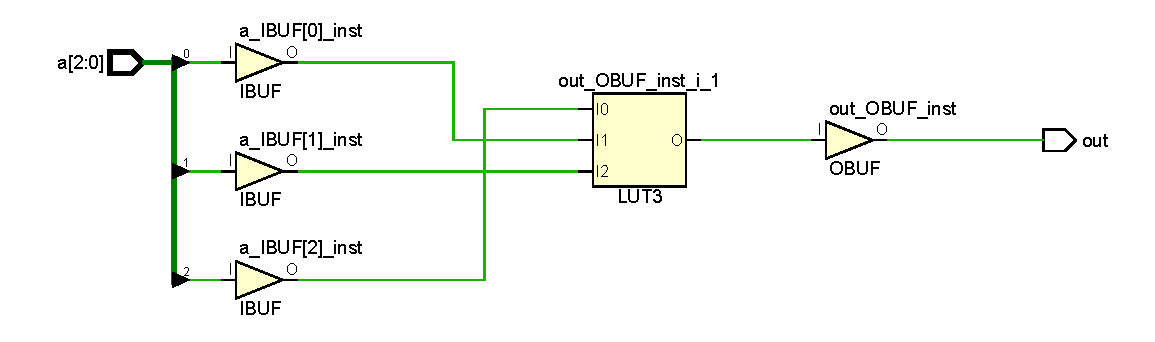
\includegraphics[width=0.9\linewidth]{figures/opt/vivado.pdf}
    }

    \subfloat[
        Yosys without optimizations enabled infers the code as a series of 2:1 MUXes.
    ]{
        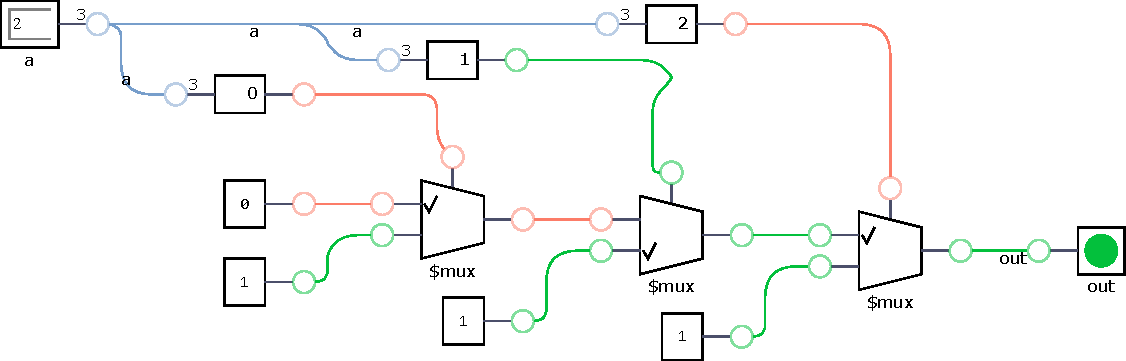
\includegraphics[width=0.7\linewidth]{figures/opt/yosys_noopt.pdf}
    }

    \subfloat[
        Yosys with optimizations enabled infers the code as one parallel OR gate.
    ]{
        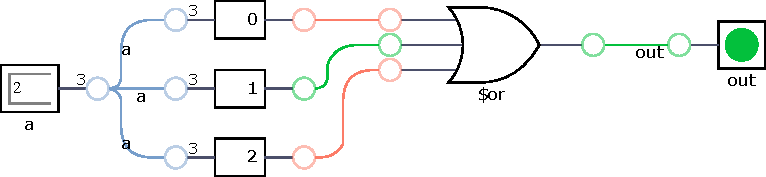
\includegraphics[width=0.7\linewidth]{figures/opt/yosys_opt.pdf}
    }

    \caption{Comparison of differences in synthesis.}
    \label{fig:opt}

\end{figure}


While synthesis tools may run their own specific optimizations, learning these intricacies are not critical, given the overall proficiency of available tools and the limited need for target-specific code optimization. Instead, the primary focus should be on teaching students to write clear and transferable code, adhering to best practices covered in the class. (See more in \autoref{section:leaderboard}.) While it is acceptable to encourage students to explore various tool and language features as illustrated in \autoref{fig:opt}, it is crucial to maintain a balance. Experimentation can stimulate curiosity and self-directed learning, but there may be instances where netlist graph viewers hinder rather than facilitate understanding. For example, as students start working with larger designs, the chances are increased that a quietly-applied, tool-specific synthesis optimization will result in a netlist that, while valid, would take too much time to decipher and understand. This may turn instructors entirely away from using netlist graph viewers due to the additional confusion that they cause. However, I argue that they are still an essential resource for introducing Verilog, helping students transition from gate schematics to HDLs. These tools serve as a foundation for students to build their intuition for synthesis, ultimately empowering them to undertake the more advanced design challenges. Even if netlist graph viewers lose their effectiveness as designs get complex, they illustrate to students the vital connection between digital design concepts and Verilog concepts.

A similar example is providing simplified schematics of transistor implementations of digital gates to relate electrical engineering students to their prior knowledge of analog design. Because transistor implementation specifics are largely unimportant due to the low demand for PDK designers, it is fine to simply introduce basic technologies such as pass-transistor logic instead of analyzing modern multi-finger FinFET CMOS designs. But only after receiving some connection to their prior experience with transistors will electrical engineering students feel comfortable working with gates. Similarly, when introducing Verilog to students, using netlist graph viewers can connect prior knowledge of digital elements to code syntax. Much like electrical engineers need some familiarity with transistor-level gate implementations prior to diving into digital design, Verilog students greatly benefit from a foundational understanding of the behavior of synthesis tools.

\FloatBarrier

\section{Rely on style guides for synthesizable SystemVerilog.}


\begin{figure}[t]
    \centering
    \frame{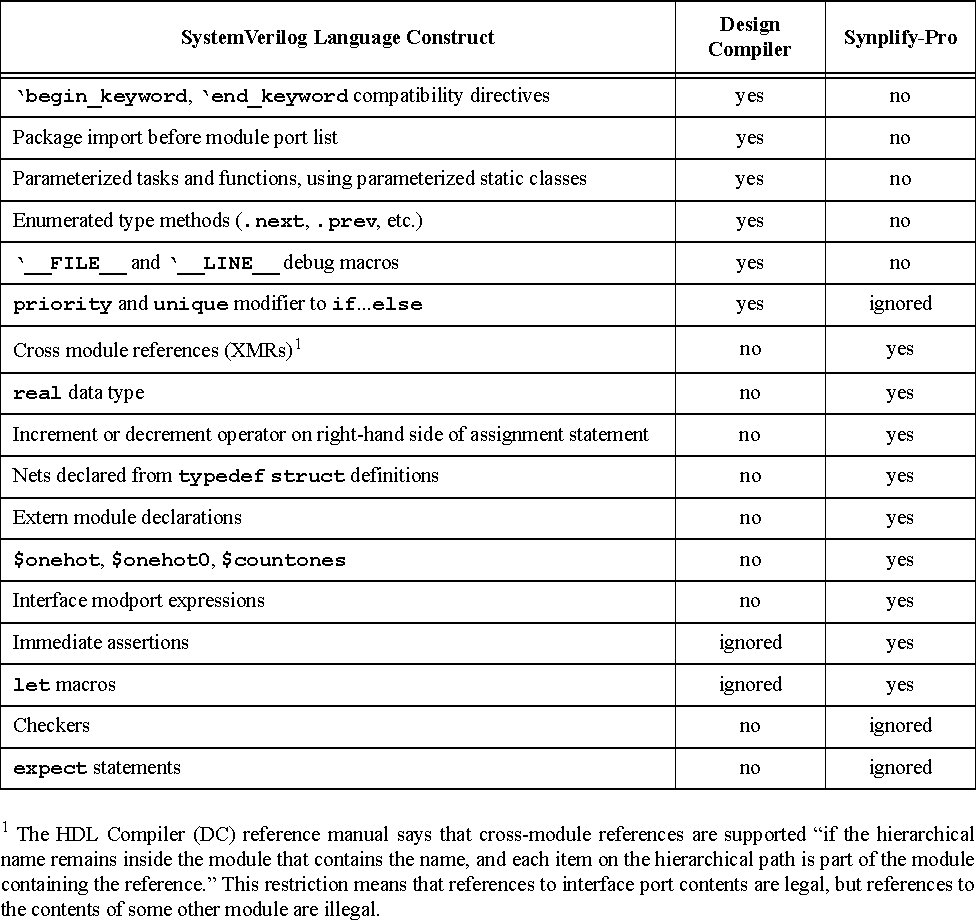
\includegraphics[width=\linewidth]{figures/dc_vs_synplify.pdf}}
    \caption{Differences in SystemVerilog Support in DC vs. Synplify-Pro from ``Synthesizing SystemVerilog: Busting the Myth that SystemVerilog is only for Verification''\cite{sutherland}}
    \label{fig:dc_vs_synplify}
\end{figure}


RTL engineers use C-like constructs [gloss] such as procedural blocks, \mintinline{systemverilog}{for} loops, and \mintinline{systemverilog}{if} statements from Verilog; and \mintinline{systemverilog}{struct}, \mintinline{systemverilog}{union}, and \mintinline{systemverilog}{enum} constructs from SystemVerilog. To promote uniformity among tools, IEEE standardized synthesis of Verilog 1364 features under the label ``1364.1". However, there has been no official ``1800.1" SystemVerilog synthesis standard to discuss the many new features that were added with SystemVerilog. With that said, many SystemVerilog features are endorsed by numerous projects and designers, as evidenced by the abundance of style guides [appx] that act as a current but unofficial documentation of SystemVerilog's synthesizable features. The SystemVerilog IEEE 1800 specification also describes many elements that are not consistently synthesizable, such as classes, hierarchical references, interfaces, and dynamic arrays \cite{1800-2017, sutherland}. This may be due to inconsistent tool-support for a feature \cite{svtests}, or that the feature is similar to a prohibited feature in the IEEE 1364.1 standard. For example, \autoref{fig:dc_vs_synplify} shows differences in synthesis support between two Synopsys synthesis tools.

\FloatBarrier

\section{It is important to teach C-like constructs that rely on inference.}


\begin{figure}[t]
    \centering

    \subfloat[
        Using purely structural constructs to create MUXes can provide long and superfluous code.
    ]{
        \begin{minipage}{0.8\textwidth}
            \footnotesize
            \inputminted[frame=single]{systemverilog}{code/c-like/low.svh}
        \end{minipage}
    }

    \subfloat[
        Using C-like constructs such as a \mintinline{systemverilog}{function}, \mintinline{systemverilog}{if} statement, and \mintinline{systemverilog}{for} loop can provide much cleaner code.
    ]{
        \begin{minipage}{0.8\textwidth}
            \footnotesize
            \inputminted[frame=single]{systemverilog}{code/c-like/high.svh}
        \end{minipage}
    }

    \caption{Comparison of purely structural Verilog versus C-like Verilog. To demonstrate this comparison, provided are two different implementations of the Find First Set operation.}
    \label{fig:c-like}

\end{figure}


A reaction to the inconsistency and ambiguity in SystemVerilog synthesis may be to teach only obviously-synthesizable constructs such as continuous assignment and standard cell initialization, but that would neglect important language features that have become popular in industry designs. Similarly, in computer programming courses, once students understand the underlying mechanisms, it is common to allow use of standard library functions and data structures. This philosophy should extend to the realm of SystemVerilog. As long as the code adheres to course-specified style guides, and students understand the resulting synthesis, higher-level syntax should be prioritized when it improves code clarity and structure. For example, observe \autoref{fig:c-like}.

\FloatBarrier

\section{HDLs can be abstractions for complex hardware concepts.}


\begin{figure}[t]
    \centering
    \inputminted[frame=single]{systemverilog}{code/cache_lab/cache.svh}
    \caption{Snippet of ``Labs with CVA6'' cache lab starter code \cite{labsWithCVA6}}
    \label{fig:cache_lab}
\end{figure}


With the full set of synthesizable features being utilized, Verilog can be a useful abstraction layer to better explain complex design concepts such as state machines, pipelining, and handshakes. This parallels the use of abstraction in programming courses, where students often draft pseudocode to conceptualize algorithms before delving into detailed implementation. Transferring this approach to digital design can promote a more rapid and comprehensive learning experience. As long as students demonstrate a strong understanding of how Verilog can be synthesized, they will also have an understanding of the circuits needed to implement the complex design concepts. An example of this in practice was in UCSB's ECE 154B, where an assignment I wrote expected students to implement a fully-associative cache. Students were expected to implement a doubly-linked-list to execute a least-recently-used replacement policy. With the helpful abstraction layer of structs, \mintinline{systemverilog}{for} loops, and \mintinline{systemverilog}{if} statements, (as seen in \autoref{fig:cache_lab}) students were able to demonstrate understanding of the LRU algorithm while also understanding the hardware that was generated.
